\documentclass{article}
\usepackage[nonatbib]{project}

\usepackage[breaklinks=true,letterpaper=true,colorlinks,citecolor=black,bookmarks=false]{hyperref}

\usepackage{amsthm}
\usepackage{amsmath,amssymb}
\usepackage{enumitem}
\usepackage{comment}

\usepackage[sort&compress,numbers]{natbib}
\usepackage[normalem]{ulem}

% use Times
\usepackage{times}
% For figures
\usepackage{graphicx} % more modern
%\usepackage{epsfig} % less modern
%\usepackage{subfig} 

\graphicspath{{../fig/}}

\usepackage{tikz}
\usepackage{tkz-tab}
\usepackage{caption} 
\usepackage{subcaption} 
\usetikzlibrary{shapes.geometric, arrows}
\tikzstyle{arrow} = [very thick,->,>=stealth]

\usepackage{cleveref}
\usepackage{setspace}
\usepackage{wrapfig}
%\usepackage[ruled]{algorithm}
\usepackage{algpseudocode}
\usepackage[noend,linesnumbered]{algorithm2e}

\usepackage{times}
\usepackage{latexsym}
\usepackage{graphicx}
\usepackage{amsfonts}
\usepackage{amsmath}
\usepackage{multirow}
\usepackage{booktabs}
\usepackage{makecell}
\usepackage{url}
\usepackage{float}

\usepackage[disable]{todonotes}

\newcommand{\red}[1]{\textcolor{red}{#1}}


\title{Analyze and Improve Cross-View Learning with Bayesian Ensemble}

\author{
	Yuqing Xie \\
	School of Computer Science\\
	University of Waterloo\\
	Waterloo, ON, N2L 3G1 \\
	\texttt{yuqing.xie@uwaterloo.ca} \\
	\And
	Peng Shi\\
	School of Computer Science\\
	University of Waterloo\\
	Waterloo, ON, N2L 3G1 \\
	\texttt{TODO@uwaterloo.ca} \\
}

\begin{document}
\maketitle
% expect the report to be less than \textbf{8 pages} (references excluded).

\begin{abstract}

Put here a brief summary of the project: what is it about, what are the related works, what is your execution plan, what do you expect to learn/contribute, and how are you going to evaluate your results. The proposal is expected to be 1 page (reference excluded), so be concise and to the point. 

\end{abstract}

\section{Introduction}

Recurrent neural networks(RNN) are now the standard method to deal with natural language. Models using long-short-term-memory(LSTM) perform extremely well on varieties of natural language tasks, ranging from machine translation, question answering to sentence classification and sentence tagging. However, unlike Convolution neural networks for vision tasks, the mechanism behind RNN is less explored and hard to visualize. Without clear understanding of the sequential models, improvements can be hard to made and further improvement will be less directed. 

Several previous work has been done to try to visualize LSTM. However, no significant findings has been made to help understand the contributions of each words. 
TODO:related works summary.
%Why can't any of the existing techniques effectively tackle this problem?

Since few theory work has been done to successfully dig deep into sequential models and apply the findings to practice, we proposed a novel method of decomposing Bi-LSTM models and visualize them for further model improvement. We decomposed trained Bi-LSTM models for sequence tagging tasks to understand the contribution of each components in the sentence. %We also improved the final model according to this finding. 
% take cross-view learning as an example in this project. We will analyze and improve cross-view learning using Bayesian ensemble.

First thought to investigate the LSTM is to watch on the contribution of each word toward the output. A clear way to do this is to apply the attention mechanism. However, what we aim to do here is not to improve the model by introducing extra weights but to just examine the existing model. We follow Jame’s to decomposition[TODO]. The main idea is to decompose the output gates in LSTM and convert them in to the contribution weights of words towards outputs. Their work focus on the sentence classification tasks -- sentiment classification. This is relative simple task and needs less understanding of the sentence structure. Contributions of each word is relatively clear according to their meaning, which can be easily represented by current word embeddings. We follow their method  made modification of their models since we focus on sequence tagging tasks and examined Bi-LSTM.

%Possible difficulties - main contribution
%How to quantify the observations and summarize it into prior knowledge.
%How to integrate the human prior knowledge in Bayesian Ensemble.

%CVT
%First let me introduce you what is cross view training. It is a semi-supervised sequence learning method. This idea first come from vision. We human can construct 3D models from slightly different views from two eyes. Even if we only look through one eye, we can still understand the world in a 3D way. That is because our brain is trained a long time to do that. Kevin Clark first brought this idea to sequence model. He took the Bi-LSTM as the primary view, which is looking through both eyes, and take each directional LSTM as partial view, which is look through only one eye. The idea of cross view training is that enabling partial views the ability to understand the whole sentence and then in tern improve the primary view, since the primary view is made up with partial views.
%Now, let’s take a closer look at cross view training. On the labeled data, Kevin followed the traditional bidirectional LSTM fashion. On the unlabeled data, Kevin followed the teacher-student fashion. We take the primary view as the teacher, and take the partial views as students. Through training, partial views will gradually learn to understand the whole sentence. However, one interesting thing here is that  in Kevin Clark’s work, they only use primary view during inference. We think the reason is that partial views are not reliable, and simply ensemble them with primary view may even add burden to the model.
%So, here comes our problem. We would like to Investigate the source of the effectiveness of cross-view training method. We will try to answer the following questions: * What does LSTM with CVT learn from the unlabeled data compared with traditional LSTM. * What is learned for different views in CVT.  And further, we wish to improve the cross-view training method based on our investigation.
%What properties did you analyze/prove about this problem or technique?

\section{Related Works}

There are mainly two lines of related work on neural network interpretability.

%TODO rewrite and summary.

First, Hendrik et al. (2016) and Karpathy et al. (2016) analyze the movement of the raw gate activations over a sequence.
Karpathy et al. (2016) is able to identify co-ordinates of $c_t$ that correspond to semantically meaningful attributes such as whether the text is in quotes and how far along the sentence a word is. However, most of the cell co-ordinates are harder to interpret, and in particular, it is often not obvious from their activations which inputs are important for specific outputs.

Another approach that has emerged in the literature Alikaniotis et al. (2016) Denil et al. (2015) Bansal et al. (2016) is for each word in the document, looking at the norm of the derivative of the loss function with respect to the embedding parameters for that word. This bridges the gap between high-dimensional cell state and low-dimensional outputs. These techniques are general- they are applicable to visualizing the importance of sets of input coordinates to output coordinates of any differentiable function. In this work, we describe techniques that are designed around the structure of LSTM’s, and show that they can give better results in that setting.

%Related work - Sequence task ensemble
%For sequential task ensemble there also exist several kinds of methods
%Rodrigues et al. (2014) proposed a CRF-based model, CRF-MA, that assumes only one annotator is correct for any given label.
%Recently, Nguyen et al. (2017) proposed an approach that outperformed CRFMA, based on hidden Markov models (HMMs),
%Both CRF-MA and HMM crowd use simpler annotator models that do not capture the effect of sequential dependencies on annotator reliability.
%Bayesian approach, which has been shown to be effective for handling uncertainty due to noise in crowdsourced data for non-sequential classification (Kim and Ghahramani, 2012; Simpson et al., 2013; Venanzi et al., 2014; Moreno et al., 2015).
%Yang et al. (2018) adapt a Bayesian neural network so that it can be trained concurrently with an annotator model.
%We will also use a Bayesian approach to aggregate primary view with partial views.

%TODO
%Summarize the range of techniques by highlighting their strengths and weaknesses  differences or limitations (if any)? 
%Suggestion: organize your summary based on desirable properties of the techniques
%What is the state of the art?
%Any open problem?

\section{Main}

To understand the mechanism behind current sequential models, we follow [TODO Ian Tenney]'s ``edge probing'' framework to construct an architectures across tasks. Unlike [Tenney] focusing on sequence classification tasks, we focus on sequence tagging problem. That is to say, given a sentence, we have to give each token a label based on the whole sentence.

\subsection{Notations}
Formally, we represent a sentence as a list of tokens $T = [t_1, t_2, ... , t_n]$, where $n$ represents the length of the sentence, and the label of each token to be $L = [l_1, l_2, ... , l_n]$. Given a sequence of tokens, we embed the tokens into a high dimension vectors. Thus, a sentence can be represented as $E = [e_1, e_2, ... , e_n], e_i \in \mathbb{R}^d, \forall 1 \leq i \leq n$, where $d$ is the embedding size. Then we pass this embedded sentence into models.

%\red{We focus on the named entity recognition task. This is to tag each word its category in terms of entity, that is does the word refer to a person, a location, an organization, etc. Usually the system needs to tag for each token their category alone with whether it is the start, inner or end part of this entity. To make future analysis easier, we simplify the task to be a binary classification task. That is to say, we classify each token to be either entity or non-entity.} 
%states twice ?

\subsection{Models}

We implement several models to compare the contribution of both embedding information and contextual information to the final prediction. 

\ 

\textbf{Uni-directional LSTM}

We follow the traditional LSTM mechanism to construct a model for sequence tagging task. Given a sequence of word embeddings, $E = [e_1, e_2, ... , e_n], e_i \in \mathbb{R}^d$, an uni-directional LSTM processes one word at a time, keeping track of cell-gates $C = [c_1, c_2, ... , c_n]$ and hidden states $H = [h_1, h_2, ... , h_n]$. After processing each token, the hidden state of current token is then passed through a fully-connected layer to form the probability distribution over classes. After a softmax activation function and argmax, the model will predict a label across classes.

In detail, each uni-LSTM cell computes $h_t$ and $c_t$ as a function of $e_t, c_{t-1}$ using the following updates. 
\begin{align}\label{eq:f1}
f_t & = \sigma(W_f x_t + V_f h_{t - 1} + b_f) \\
i_t & = \sigma(W_i x_t + V_i h_{t - 1} + b_i) \\
o_t & = \sigma(W_o x_t + V_o h_{t - 1} + b_o) \\
\tilde{c}_t & = \tanh(W_c x_t + V_c h_{t - 1} + b_c) \\
c_t & = f_t \odot c_{t - 1} + i_t \odot \tilde{c}_t \\
h_t & = o_t \odot \tanh(c_t)
\end{align}

As initial values, we define $c_0=h_0=0$. 
Then the probability distribution for the $t$ th token for the $c$ th class is specified by $p_{t, c} = \text{SoftMax}(W h_t) = \frac{e^{W_{:c} h_t}}{\sum_{j = 1} ^ C e^{W_{:j} h_t}}$, where $W_{:j}$ is the $i$ th row of the matrix $W$.

This is the forward directional LSTM. In this case, the information is passed from the beginning of the sentence to the end. We also consider the backward directional LSTM for later comparison. The only difference will be the update direction and the initial value. The initial values are assigned to $c_n=h_n=0$. And the information is passed from the end of the sentence to the beginning, which means we update the $t$ th token using the $t+1$ th token instead of the $t-1$ th as in the forward version.
%\begin{align}
%f_t & = \sigma(W_f x_t + V_f h_{t + 1} + b_f) \\
%i_t & = \sigma(W_i x_t + V_i h_{t + 1} + b_i) \\
%o_t & = \sigma(W_o x_t + V_o h_{t + 1} + b_o) \\
%\tilde{c}_t & = \tanh(W_c x_t + V_c h_{t + 1} + b_c) \\
%c_t & = f_t \odot c_{t _ 1} + i_t \odot \tilde{c}_t \\
%h_t & = o_t \odot \tanh(c_t)
%\end{align}

\ 

\textbf{Bi-directional LSTM}

Uni-directional LSTM networks suffer from only seeing information from one side of the sentence. So we also include a bi-directional LSTM to examine the information learnt from both sides. The encoding process is just simply concatenate forward and backward gates together. We demote the forward gates as $f_t^{fw}, i_t^{fw}, o_t^{fw}, c_t^{fw}, h_t^{fw}$, and the backward gates as $f_t^{bw}, i_t^{bw}, o_t^{bw}, c_t^{bw}, h_t^{bw}$. We also demote the concatenated matrix of $*_t^{fw}$ and $*_t^{bw}$ as $[*_t^{fw}, *_t^{bw}]$. After concatenate the forward and backward gates together, using $[*_t^{bw}, *_t^{fw}]$ to replace $*_t$ in formulas of \ref{eq:f1}, we can represent the update formulas in a same form. 

Also probability distribution for the $t$ th token for the $c$ th class is specified by $p_{t, c} = \text{SoftMax}(W [h_t^{fw}, h_t^{bw}]) = \frac{e^{W_{:c} [h_t^{fw}, h_t^{bw}]}}{\sum_{j = 1} ^ C e^{W_{:j} [h_t^{fw}, h_t^{bw}]}}$,.

\ 

\textbf{MLP}

To examine what information has been learnt by LSTM from the context and what information can be directly learned from the word embedding, we also implemented a 2-layer MLP network to tag the tokens only according to the embeddings. Each MLP layer can be represented as follow:
The input of the $i$ th layer is represented as $x_i$, then the $i$ th layer is $f_i(x_i) = \sigma(W_i x_i + b_i)$, where $W_i$ and $b_i$ are the weights and bias of the $i$ th layer. In this work we use ReLU as our activation function $\sigma$. Then the output of the $i$ th layer $f_i(x_i)$ is then feed into the next layer as input. That is to say $x_{i+1} = f_i(x_i)$. In this implementation, we use a 2-hidden-layer MLP.

We compared the four different embeddings: the original pre-trained embedding from Glove, the tuned embedding of forward and backward uni-directional LSTM and the bi-directional LSTM. The final probability will be $p_{t, c} = \text{SoftMax}(f_3(e_t))$.% explain more?

\subsection{Decomposition}

\textbf{Uni-LSTM}

We now show that we can decompose the numerator of $p_{t, c}$ into a product of factors, and interpret those factors as the contribution of individual words of the predicted probability of class $c$ for uni-LSTM. Also taking the forward direction as an example, define 
\begin{equation}\label{eq:uni-beta} 
\beta_{t, c, j} = \exp\left(W_{:c} (o_t \odot (\tanh(c_j)- \tanh(c_{j-1}))\right),
\end{equation}
so that 
\[\exp( W_{:c} h_t) = \exp\left(\sum_{j=1}^t W_{:c} (o_t \odot (\tanh(c_j) - \tanh(c_{j-1}))\right) = \prod_{j=1}^t \beta_{t, c, j}.\]

As $\tanh(c_j) - \tanh(c_{j-1})$ can be viewed as the update resulting from word $j$, so $\beta_{t, c, j}$ can be interpreted as the multiplicative contribution to $p_{t, c}$ by word $j$. 

This is a direct extension of [TODO]'s work, in which we expand their method to suit sequence tagging tasks.
The backward direction will just be the same.

\textbf{Bi-LSTM}

For the bi-directional LSTM decomposition, we can simply de-concatenate the gate states and compute the contribution of each direction as in the uni-direction version. Then each token's probability distribution can be taken as a combination of both direction. That is to say, the probability can be interpreted as follow:
\begin{align}\label{eq:bi-beta} 
\beta_{t, c, j} = \exp(&W_{:c} [h_t^{fw}, h_t^{bw}])\\
= \exp(&W_{:c}^{fw} (o_t^{fw} \odot (\tanh(c_j^{fw})- \tanh(c_{j-1}^{fw}))) \\
+ &W_{:c}^{bw} (o_t^{bw} \odot (\tanh(c_j^{bw})- \tanh(c_{j+1}^{bw})))),
\end{align}
Let
\begin{equation}
\beta_{t, c, j}^{fw} = \exp(W_{:c}^{fw} (o_t^{fw} \odot (\tanh(c_j^{fw})- \tanh(c_{j-1}^{fw}))))
\end{equation}
and
\begin{equation}
\beta_{t, c, j}^{bw} = \exp(W_{:c}^{bw} (o_t^{bw} \odot (\tanh(c_j^{bw})- \tanh(c_{j+1}^{bw}))))
\end{equation}
so that 
\begin{equation}
\beta_{t, c, j} = \beta_{t, c, j}^{fw} \beta_{t, c, j}^{bw}
\end{equation}
Then we have:
\begin{align}
	\exp(&W_{:c} [h_t^{fw}, h_t^{bw}]) \\
= \exp(&\sum_{j=1}^t W_{:c}^{fw} (o_t^{fw} \odot (\tanh(c_j^{fw}) - \tanh(c_{j-1}^{fw}))) +\\
	&\sum_{j=t}^n W_{:c}^{bw} (o_t^{bw} \odot (\tanh(c_j^{bw}) - \tanh(c_{j+1}^{fw}))))\\
= \prod_{j=1}^t &\beta_{t, c, j}^{fw} \prod_{j=t}^n \beta_{t, c, j}^{bw}.
\end{align}

\begin{comment}
\subsection{An Additive Decomposition of the LSTM cell}

We will show below that the $\beta_{i,j}$  capture some notion of the importance of a word to the LSTM's output.   However, these terms fail to account for how the information contributed by word $j$ is affected by the LSTM's forget gates between words $j$ and $T$. Consequently, we empirically found that the importance scores from this approach often yield a considerable amount of false positives. A more nuanced approach is obtained by considering the additive decomposition of $c_T$ in equation \eqref{eq:additive}, where each term $e_j$ can be interpreted as the contribution to the cell state $c_T$ by word $j$. By iterating the equation $c_t = f_tc_{t - 1} + i_t \tilde{c}_t$, we get that
\begin{equation}
c_T = \sum_{i=1}^T (\prod_{j=i + 1}^T f_j) i_i \tilde{c}_i = \sum_{i=1}^T e_{i, T} \label{eq:additive}
\end{equation}
This suggests a natural definition of an alternative score to the $\beta_{i, j}$, corresponding to augmenting the $c_j$ terms with products of forget gates to reflect the upstream changes made to $c_j$ after initially processing word $j$. 
\begin{align}
\label{eq:gamma}
\exp(W_i h_T) & = \prod_{j=1}^T \exp \left( W_i(o_T \odot (\tanh(\sum_{k = 1}^j e_{k, T}) - \tanh(\sum_{k=1}^{j - 1}e_{k, T})))\right) \\
& = \prod_{j=1}^T \exp \left( W_i(o_T \odot (\tanh((\prod_{k=j+1}^t f_k) c_j) - \tanh((\prod_{k=j}^t f_k) c_{j - 1}))) \right) \\
& = \prod_{j=1}^T \gamma_{i,j}
\end{align}
\section{Phrase Extraction for Document Classification}
We now introduce a technique for using our variable importance scores to extract phrases from a trained LSTM. To do so, we search for phrases which consistently provide a large contribution to the prediction of a particular class relative to other classes. The utility of these patterns is validated by using them as input for a rules based classifier. For simplicity, we focus on the binary classification case.
\subsection{Phrase Extraction}
\label{sec:phrase_extraction}
A phrase can be reasonably described as predictive if, whenever it occurs, it causes a document to both be labelled as a particular class, and not be labelled as any other. As our importance scores introduced above correspond to the contribution of particular words to class predictions, they can be used to score potential patterns by looking at a pattern's average contribution to the prediction of a given class relative to other classes. More precisely, given a collection of $D$ documents $\{\{x_{i,j}\}_{i = 1}^ {N_d} \}_{j=1}^D$, for a given phrase $w_1,...,w_k$ we can compute scores $S_1, S_2$ for classes 1 and 2, as well as a combined score $S$ and class $C$ as
\begin{align}
S_1(w_1,...,w_k) & =  \frac{\text{Average}_{j,b}\left\lbrace \prod_{l=1}^k \beta_{1, b + l, j} | x_{b + i, j} = w_i, i = 1,...,k  \right\rbrace}{\text{Average}_{j,b}\left\lbrace \prod_{l=1}^k \beta_{2, b + l, j} | x_{b + i, j} = w_i, i = 1,...,k  \right\rbrace} \\
S_2(w_1,..,w_k) & = \frac{1}{S_1(w_1,...,w_k)} \\
S(w_1,...,w_k) & = \max_i(S_i(w_1,...,w_k))\\
C(w_1,...,w_k) & = \text{argmax}_i(S_i(w_1,...,w_k))
\end{align}
where $\beta_{i, j, k}$ denotes $\beta_{i, j}$ applied to document $k$. 

The numerator of $S_1$ denotes the average contribution of the phrase to the prediction of class 1 across all occurrences of the phrase. The denominator denotes the same statistic, but for class 2. Thus, if $S_1$ is high, then $w_1,...,w_k$ is a strong signal for class 1, and likewise for $S_2$. We propose to use $S$ as a score function in order to search for high scoring, representative, phrases which provide insight into the trained LSTM, and $C$ to denote the class corresponding to a phrase.

In practice, the number of phrases is too large to feasibly compute the score of them all. Thus, we approximate a brute force search through a two step procedure. First, we construct a list of candidate phrases by searching for strings of consecutive words $j$ with importance scores $\beta_{i,j} > c$ for any $i$ and some threshold $c$; in the experiments below we use $c=1.1$. Then, we score and rank the set of candidate phrases, which is much smaller than the set of all phrases. 

\subsection{Rules based classifier}

The extracted patterns from Section \ref{sec:phrase_extraction} can be used to construct a simple, rules-based classifier which approximates the output of the original LSTM. Given a document and a list of patterns sorted by descending score given by $S$, the classifier sequentially searches for each pattern within the document using simple string matching. Once it finds a pattern, the classifier returns the associated class given by $C$, ignoring the lower ranked patterns. The resulting classifier is interpretable,  and despite its simplicity,  retains much of the accuracy of the LSTM used to build it.
\end{comment}

%formulate your problem precisely (mathematically), present the technical challenges (if any), discuss the tools or datasets that you will build on, state your goals, and come up with a plan for evaluation.

\section{Experimental Setup}

We conduct extensive experiments to answer the question: What do the Bi-LSTM learn? 


\subsection{Dataset} Our experiments are conducted based on OntoNotes 5 English dataset~\cite{weischedel2012ontonotes}, focusing on Entity Detection task. The Entity Detection task is usually formulated as a sequence labeling task: labels are assigned to each token. Different tagging scheme can be adopted, such as \textit{BIO}, \textit{BIOES}, etc. For simplification, in this work, we use \textit{IO} scheme: if the token is a part of entity, it will be annotated as \textbf{I}; otherwise, it will be annotated as \textbf{O}. One special case that this tagging scheme can not handle is that two entity appear consecutively in one sentence, because there is not boundary label such \textbf{B}~(begin of entity). So in our experiments, we remove the sentences with consecutive entities for further experiments. The performance is evaluated by Precision, Recall and F1 scores.

\subsection{Hyper-parameters}


\subsection{Setup}

To investigate the problem: What does the Bi-LSTM learn, we decompose it into three small problems:

\begin{itemize}
	\item Does Bi-LSTM perform significantly better than Uni-directional LSTM and local models such as MLP? In what cases, Bi-LSTM is better than uni-directional LSTM and local models? And in what cases, Uni-directional LSTM and local models can also work well?
	\item How to verify that the Bi-LSTM model learn to do prediction based on contextual information?
	\item Why do Uni-directional LSTM and local model also work in some cases? 
\end{itemize}

To answer first question, we conduct the experiments with Bi-LSTM, Uni-directional LSTM model. The embedding is initialized with GloVe pretraining embeddings~\cite{pennington2014glove}. To investigate what kind of information gain provided by the LSTM, we also conduct experiments with MLP. We adopt the fine-tuned embeddings in LSTM and fix them during the training of MLP model. This is known as probing technique. 

To answer the second question, we use the LSTM decomposition technique to further investigate the contribution distribution for the token level prediction. The decomposition is conducted for Bi-LSTM and Uni-directional LSTM. 

To answer the third question, we leverage visualization techniques such as t-SNE~\cite{maaten2008visualizing}, to visualize the hidden vectors.

\section{Results}

We demonstrate our results regarding different questions we are trying to answer. 


\subsection{Question 1}

\begin{table}[t]
	\centering
	\begin{tabular}{l@{\qquad}ccc}
		\toprule
		\textbf{Model}         & \textbf{Precision} & \textbf{Recall} & \textbf{F1} \\ \midrule
		Bi-LSTM &  84.82 & 83.60  & 84.20 \\
		Uni-LSTM & 72.47 & 73.88 & 73.17 \\
		MLP(bi) & 54.97 & 75.65 & 63.67 \\ 
		MLP(uni) & 60.80 & 61.75 &  61.27 \\ 
		\bottomrule
	\end{tabular}
	\vspace{3mm}
	\caption{Entity Detection performance on OntoNotes 5 English Dataset Test set. Uni-LSTM denotes the Uni-directional LSTM. MLP(bi) denotes the MLP model based on the Bi-LSTM embeddings. MLP(uni) denotes the MLP model based on Uni-directional LSTM embeddings.}
	\label{res:ner}
\end{table}


\noindent \textbf{Bi-LSTM v.s. Uni-LSTM}


The experiment results are shown in Table~\ref{res:ner}. Compare the effectiveness of Bi-LSTM model and Uni-LSTM model, we can observe that Bi-LSTM has better F1 score~(+11.03) than the Uni-LSTM model, which is a large gap in Entity Detection task. To order to quantify what kind of error does Uni-LSTM make, we conduct further error analysis. We select those examples that Bi-LSTM makes correct predictions and but Uni-LSTM fails, and further categorize them into \red{n} types, as shown in \ref{}.
%{'EOETrue': 823, 'EOEFalse': 214, 'OEOTrue': 239, 'OEOFalse': 117}
\begin{table}[t]
\centering\centering\resizebox{\columnwidth}{!}{
\begin{tabular}{llp{10cm}}
\hline\hline
category		& number	&examples \\
OEOTrue		&14		& For \textbf{more} information check out : www.taconet.com.tw/cstudio/\\
OEOFalse		&10		& Dr. Konan Peck , an assistant research fellow at Academia Sinica 's Institute of Biomedical Sciences -LRB- IBMS -RRB- , says that \textbf{biochips} need to be made more widely available as a molecular biology research tool .\\
EOETrue		&38		& In \textbf{the} first quarter of this year , the development of Guangzhou 's privately owned enterprises again showed many characteristics : all walks of life are developing extensively , and the development of industry and commerce is remarkable .\\
EOEFalse		&13		& \textbf{Guofang} Shen said that this bill is a bill carrying political discrimination and extremely unfriendly to China .\\
\hline
Embedding	&2		& \textbf{Thick} fog , rain and high winds are limiting visibility at the site .  \\
False		& 11		& Even if you wanted to , you wo n't be reading \textbf{Jermaine} 's account now.\\
Nearby 		& 51		&Ah , yes , something called \textbf{a} Star Chamber .\\
Others		& 9		&And although Pennsylvania and Massachusetts suffered slight declines \textbf{earlier} in the decade , they are growing again .\\
\hline
\end{tabular}}
\label{tab:bi-uni}
\caption{Statistic of Bi-LSTM and uni-LSTM comparison.}
\end{table}


\noindent \textbf{Bi-LSTM v.s. MLP(bi)}

Further comparing the results of Bi-LSTM and MLP(bi), we can better understand the gains brought by the Bi-LSTM contextual encoding layer. Even leveraging the embeddings learned in Bi-LSTM model, the fine-tune MLP model still falls far behind the Bi-LSTM model. This comparison proves that the Bi-LSTM indeed empowers the entity detection ability. Further error analysis is shown in \red{tab:bi-mlp}.

\begin{table}[t]
\centering\centering\resizebox{\columnwidth}{!}{
\begin{tabular}{llp{10cm}}
\hline\hline
category		& number	&examples \\
OEOTrue		&14		& \textbf{Electrical} and high science and technology products grew considerably.\\
OEOFalse		&47		& Another popular technique involves covering the trees with black \textbf{mosquito} nets to improve yields.\\
EOETrue		&34		& David any reaction from the Bush team on the Democrats ' plan to contest the vote in Miami \textbf{-} Dade?\\
EOEFalse		&0		& - \\
\hline
Embedding	&13		&  \textbf{Consumer} activists are skeptical. \\
False		& 46		& I forced myself to refrain from the grief of \textbf{loosing} my beloved car -LRB- mine was liability - only coverage -RRB- and asked the friend to send their family home.\\
Inner 		& 20		& It says that what \textbf{the} North Koreans did was a threat to international peace and security.\\
Others		& 16		& It achieved a total volume of 4 billion US dollars of goods going into and out of the area , increasing by 83 \% over \textbf{the same period of the previous} year , with a total amount of 1 billion US dollars from imports and exports.\\
\hline
\end{tabular}}
\label{tab:bi-mlp}
\caption{Statistic of Bi-LSTM and MLP comparison.}
\end{table}


\noindent \textbf{Uni-LSTM v.s. MLP(uni)}





\subsection{Question 2}

In question 1, we have empirically shown that the LSTM model could perform significantly better than local model, then we also want to show this in more theoretically way. With LSTM decomposition, we find that the LSTM can correct several errors made by local model such as MLP. 





\subsection{Question 3}

\begin{figure}[t]
	\centering
	\begin{subfigure}{0.5\textwidth}
		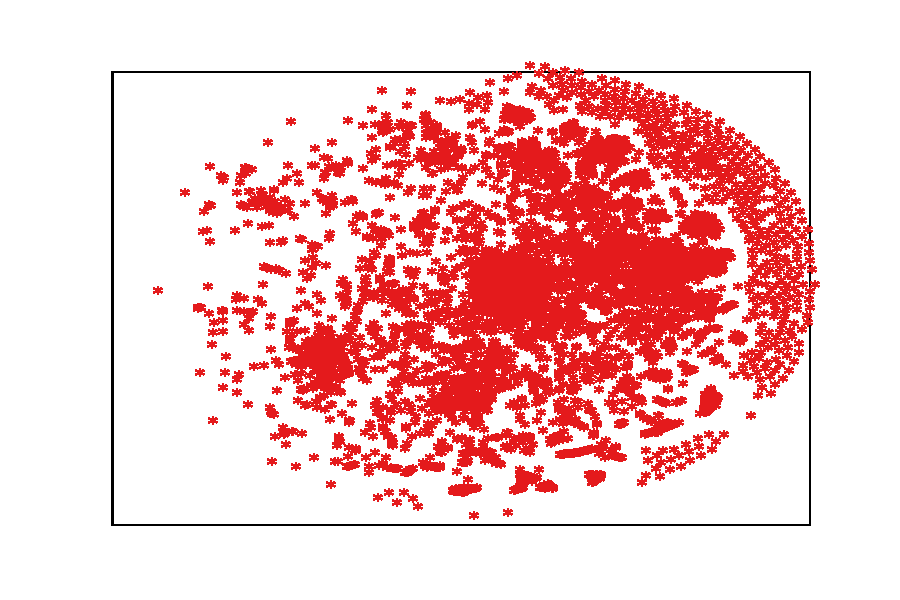
\includegraphics[width=\linewidth]{glove_embedding_positive.pdf}
		\caption{Glove Embedding with entity word}
		\label{fig:glove_positive}
	\end{subfigure}\hfil 
	\begin{subfigure}{0.5\textwidth}
		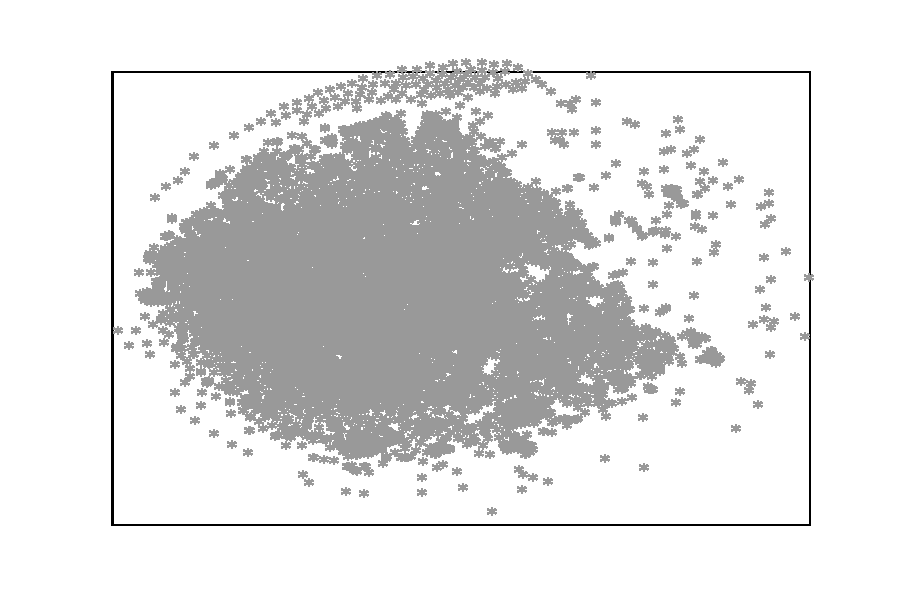
\includegraphics[width=\linewidth]{glove_embedding_negative.pdf}
		\caption{Glove Embedding with non-entity word}
		\label{fig:glove_negative}
	\end{subfigure}
\end{figure}

We can observe that with local model such as MLP(bi) or MLP(uni), the model can also achieve reasonable performance. More than 60 F1 score can be obtained by simple local model. In this subsection, we are trying to investigate the reason behind this, mainly focusing on the embedding level. 

We firstly classify the word into two categories: words belong to at least one entity~(entity word), and words nerve belong to any entity(non-entity word). We leverage the t-SNE to decompose the any embeddings into two dimensions with unit axises and visualize it. In the following figures, red dots denote entity words and grey dots denote non-entity words. 

We firstly decompose the original GloVe embedding, as shown in Figure~\ref{fig:glove_positive} and Figure~\ref{fig:glove_negative}. We can observe that most of the entity word and non-entity word are mix in the middle of the figures. 


% We first trained a Bi-LSTM model for NER task on the CoNLL-2003 dataset (Tjong Kim Sang and De Meulder, 2003). It is a classic dataset for NER(TODO, more description). Then we applied the described method above to decompose the model. The contribution weights can be visualized as follow.

%Describe the datasets you tested on; justify their relevance
%Compare empirically the techniques for complexity, performance, ease of use, etc.
%Analyze and compare (empirically or theoretically) your new approach to existing approaches
%What is the best technique, in terms of what?
%Is any technique good enough to declare the problem solved?
 
\section{Results}



\section{Conclusion}
%Can your new technique effectively tackle the problem?
%What future research do you recommend?

%\section*{Acknowledgement}
%Thank people who have helped or influenced you in this project.

\nocite{*}

\bibliographystyle{unsrtnat}

\bibliography{project}

\end{document}